% E1 manuscript — Journal of Process Control (elsarticle)
% Compile: see compile.bat / README. Easiest path: upload manuscript/latex/,
% figures/, and literature/references.bib to Overleaf as one project.
\documentclass[review,number,sort&compress]{elsarticle}

\usepackage{graphicx}
\usepackage{amsmath,amssymb}
\usepackage{booktabs}
\usepackage[colorlinks=true,allcolors=blue]{hyperref}
\graphicspath{{../../figures/}}

\journal{Journal of Process Control}

\begin{document}
\begin{frontmatter}

\title{A credibility-weighted hybrid soft sensor and uncertainty-consuming
robust real-time optimization for silica scaling control in Philippine
geothermal fields: design, negative results, and out-of-sample
validation}

% AUTHOR METADATA (confirmed by author): sole author, no adviser
% (independent thesis). Affiliation: University of the Philippines
% Diliman (author decision, 2026-11-05).
\author[upd]{Bien Don Busico}
\ead{bienbusico@gmail.com}
\affiliation[upd]{organization={University of the Philippines Diliman},
city={Quezon City}, country={Philippines}}

\begin{abstract}
Scaling processes couple strongly nonlinear kinetics to hard operational
constraints, and the models available for them are structurally wrong in
ways that matter. In this work the wrongness is measured rather than
assumed: a classical fitted rate law mispredicts independent modern
kinetic data by a factor of six at the median. We present a control
architecture that treats such mismatch as a first-class design object.
A hybrid soft sensor combines a physics core with a learned residual
whose weight is set by its own leave-one-out credibility, so the
correction fades back to the prior whenever the data has not earned it.
A vertex-robust economic real-time optimizer then consumes both the
correction and its uncertainty, the latter as a multiplicative
constraint back-off. On a synthetic brine-line plant grounded in the
primary-literature chemistry of Philippine liquid-dominated geothermal
fields, the sensor reduces estimation error by 40\% relative to physics
alone and 48\% relative to a purely data-driven model under sparse
daily labels. In closed loop it is the only tested policy that remains
essentially violation-free in two regimes: benign random mismatch
(+33\% power uplift, zero violation days) and an adverse stress set at
the measured sixfold kinetic gap (0.5 post-warm-up violation days
against 17.2 for the robust open loop). Two pre-registered failures,
of zero-shot residual transfer and of scalar modifier adaptation
against multiplicative mismatch, motivated the design and are reported
as results. Every kinetic, solubility and sensing component is
validated out-of-sample against an independent 2024 experimental
dataset.

\end{abstract}

\begin{keyword}
soft sensor \sep hybrid modeling \sep real-time optimization \sep
plant--model mismatch \sep geothermal energy \sep silica scaling \sep
Philippines
\end{keyword}

\end{frontmatter}

\section{Introduction}\label{sec:intro}

Process models tend to be wrong precisely where constraints bind. This
paper works through a case in which the wrongness can be put on a
scale. The classical kinetic law for amorphous-silica polymerization,
transcribed faithfully from its 1979 primary source, mispredicts the
effective decay rate observed in an independent 2024 laboratory corpus
by a factor of six at the median. Yet silica scaling must be managed
daily and at industrial scale. In the liquid-dominated geothermal
fields of the Philippines, which rank among the largest installed
capacities in the world~\citep{fronda2020country}, dissolved silica
sets the floor on reinjection temperature and therefore the ceiling on
bottoming-cycle power. Mitigation practice at the Bacman- and
Tiwi-type fields that motivate this study is documented and static:
fixed inhibitor programs and manually managed reinjection
temperatures~\citep{see2010wgc,remoroza2008ph,baltazar2014grc,%
kobayashi2024mahanagdong}. Between a model too wrong to trust and a
practice too static to optimize sits the control problem addressed
here.

The individual ingredients are established. Machine-learned predictors
of geothermal scaling exist in prediction-only
form~\citep{juhri2024sgw}. Hybrid physics--data modeling has a mature
canon~\citep{psichogios1992hybrid,thompson1994modeling,%
vonstosch2014hybrid,karniadakis2021physics}, soft-sensor practice under
sparse labels is well codified~\citep{kadlec2009data}, and real-time
optimization under plant--model mismatch has a developed theory of
modifier adaptation~\citep{marchetti2009modifier,marchetti2010dual,%
darby2011rto}. What has been missing, and what a constraint with
fourth-power sensitivity punishes, is the coupling between them: an
estimator that knows how much of its own learned correction to believe,
and an optimizer that spends that belief as constraint margin. Two
pre-registered negative results in this paper show that the coupling is
not a refinement but a requirement. A residual transferred across
plants actively harms, and a scalar bias adaptation, the natural first
recourse, cannot stabilize a multiplicative kinetic error on a
fourth-power constraint even while it harvests spectacular nominal
profit.

The contributions are fivefold. First, a credibility-weighted hybrid
soft sensor whose leave-one-out shrinkage yields provable graceful
degradation to its physics prior and doubles as the deployment safety
interlock. Second, a vertex-robust economic real-time optimizer that
consumes the sensor's correction together with its cross-validated
uncertainty as a multiplicative back-off. Third, a two-regime
closed-loop evaluation, spanning benign random mismatch and an adverse
stress set at the measured sixfold gap, that maps a safety--harvest
frontier on which the proposed loop is the only policy essentially free
of violations in both regimes. Fourth, out-of-sample validation of
every physics component and of the sensing pattern itself against the
independent 2024 corpus, which yields a reconciliation of second-order
decay with the classical fourth-order peak-rate law, a mutual
solubility validation at a median of $1.05\times$, and a design
principle we state as: identifiability precedes correction. Fifth, a
fully specified and regenerable benchmark problem, built on
Philippine-field chemistry, with a quartic constraint, an induction
delay, a non-monotonic actuator and a $\times 101$ temperature lever,
offered to the constrained-optimization community.

Section~\ref{sec:benchmark} states the problem and its industrial
context, Section~\ref{sec:arch} the architecture,
Section~\ref{sec:results} the in-silico results,
Section~\ref{sec:validation} the out-of-sample validation, and
Section~\ref{sec:discussion} the limitations and what generalizes.

\section{The scaling-control problem as a benchmark}\label{sec:benchmark}

\subsection{Philippine industrial context}\label{sec:phcontext}

The Philippines operates among the world's largest installed geothermal
capacities, dominated by liquid-dominated fields whose separated brines
leave the flash plant at or near amorphous-silica
saturation~\citep{fronda2020country}. Polymerization of that silica
sets the effective floor on reinjection temperature, and with it the
ceiling on bottoming-cycle heat recovery, across fields of the Bacman
and Tiwi type whose chemistry anchors this work. The endmember brine
envelope is taken from the Tiwi geochemical
survey~\citep{sugiaman2004geochemical}; twenty years of geochemical
records at Bacman document how far a single field's chemistry can
wander over an operating life~\citep{espartinez2015bacman}.

Mitigation practice at these fields is documented and, importantly for
what follows, static. The record includes inhibitor hot-injection
trials at BacMan-II~\citep{see2010wgc}, field tests of pH
modification~\citep{remoroza2008ph}, a sustained phosphino-carboxylate
inhibitor program~\citep{baltazar2014grc}, and manual management of
reinjection lines~\citep{kobayashi2024mahanagdong}. These programs form
the empirical baseline against which our controller is benchmarked;
none of them closes a model-based loop. Economic quantities throughout
are peso-denominated, with every coefficient declared as a scenario
band. Where trade-press figures inform a scenario, notably the
400~kg/s Bacman-scale brine stream, they set scale only and are never
fitted to or used as validation targets; the repository enforces this
rule in code.

\subsection{Chemistry as control structure}\label{sec:chemistry}

Read in control language, silica scaling is a constraint process with
four features that together make it a demanding benchmark for economic
optimization under mismatch. The classical rate correlation is a
fourth-order peak-rate law in
supersaturation~\citep{rothbaum1979rohde}, so modest errors in
chemistry or temperature are raised to the fourth power exactly where
the constraint binds. The rate constant is non-Arrhenius above roughly
90~$^{\circ}$C: a low-temperature Arrhenius fit ($E_a = 9.1$~kJ/mol
over 5--90~$^{\circ}$C) overpredicts $k$ at 150~$^{\circ}$C by a factor
of 3.0 (Fig.~\ref{fig:arrhenius}), which means extrapolating cold-lab
kinetics to a hot brine line is quantitatively wrong rather than merely
imprecise. The process carries an induction delay, with onset lagging
supersaturation exposure and the induction period falling steeply in
supersaturation ($P \propto s^{-4.3}$, $r^2 = 0.88$, fitted from the
same primary dataset). Finally, the inhibitor actuator is
non-monotonic~\citep{gallup2002investigations}: the best organic
formulation suppressed deposition by more than half near 1~ppm, and
inhibition then decreased at higher dosage. Dosing is therefore a
genuine optimization problem, not a saturating knob.

Solubility sets the economic stakes of the temperature lever. Using the
primary amorphous-silica correlation of \citet{gunnarsson2000amorphous}
with the Tiwi archetype brine, cooling the reinjection line from 150 to
90~$^{\circ}$C raises the uninhibited polymerization rate by a factor
of about 101 (Fig.~\ref{fig:lever}). Every degree of additional heat
recovery is purchased at a steeply nonlinear scaling price, which is
why a static policyleaves either megawatts or safety margin on the
table.

\begin{figure}[t]\centering
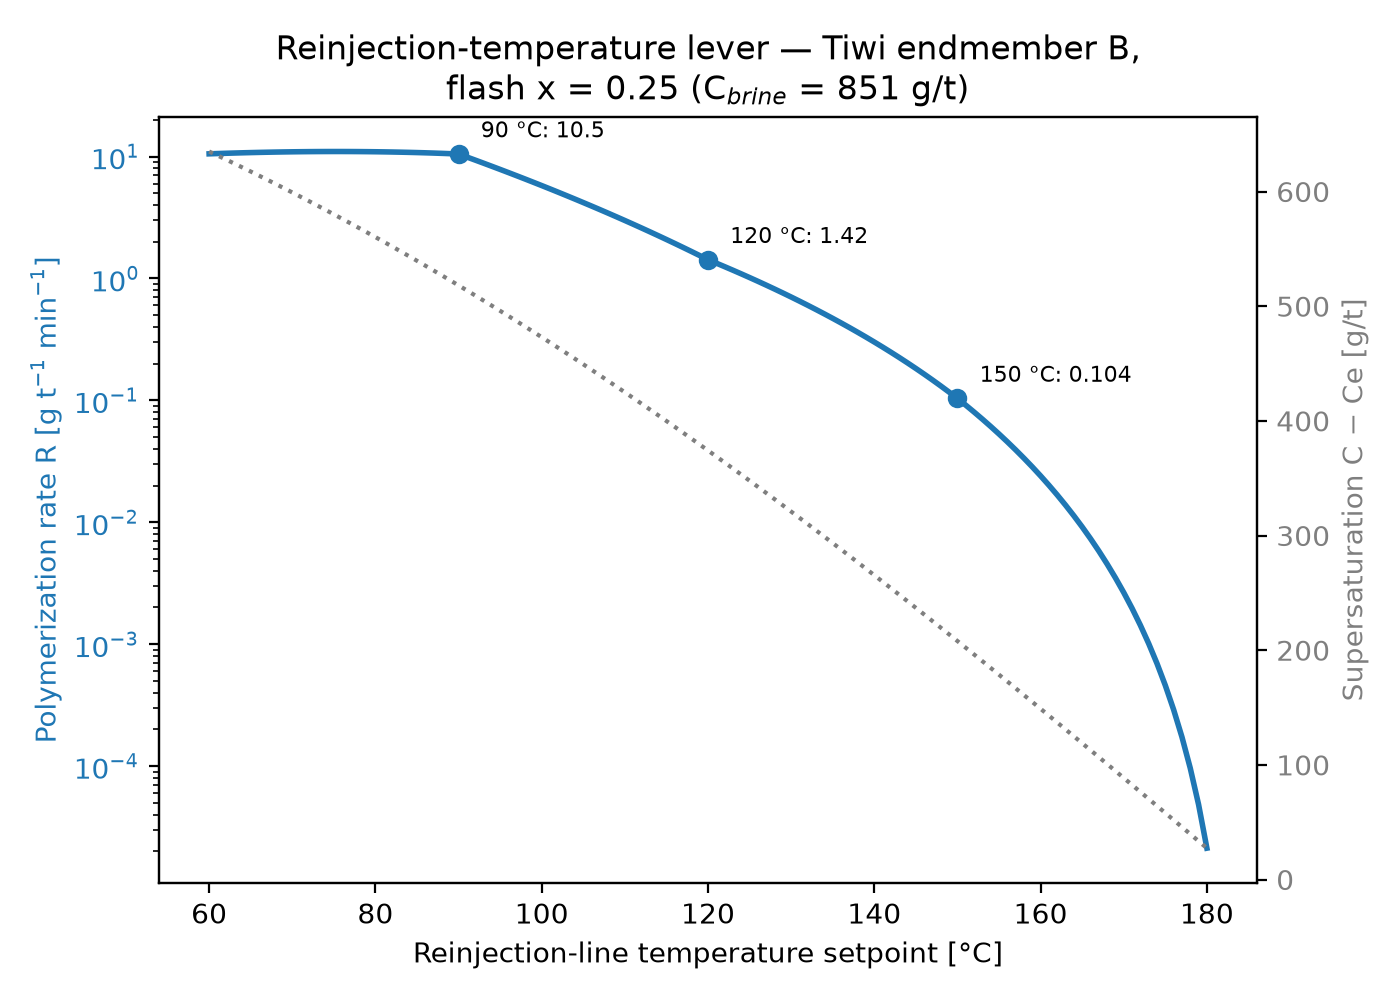
\includegraphics[width=.72\linewidth]{fig_temperature_lever.png}
\caption{The reinjection-temperature lever. Uninhibited polymerization
rate along the brine line versus temperature set-point for the
archetype brine (Tiwi endmember B, 638~mg/kg reservoir
silica~\citep{sugiaman2004geochemical}; flash fraction $x = 0.25$,
scenario input; solubility from \citet{gunnarsson2000amorphous};
kinetics from the checksum-validated transcription of
\citet{rothbaum1979rohde}). Cooling from 150 to 90~$^{\circ}$C raises
the rate by a factor of 101.}\label{fig:lever}
\end{figure}
\begin{figure}[t]\centering
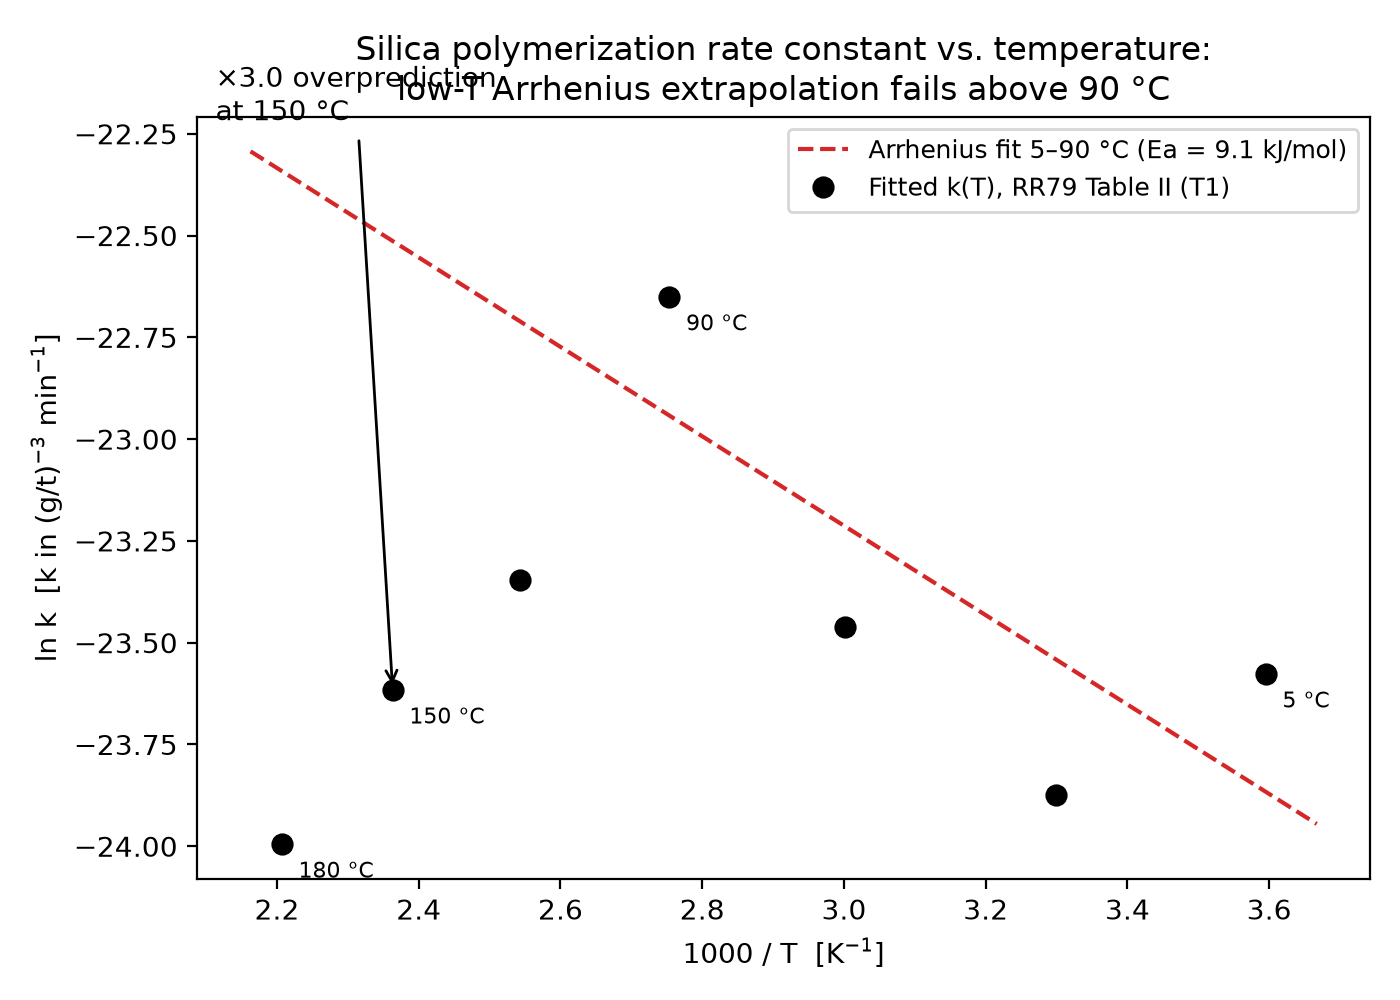
\includegraphics[width=.72\linewidth]{fig_arrhenius_overprediction.png}
\caption{Fitted fourth-order rate constants $k(T)$ over
5--180~$^{\circ}$C, regenerated from the primary transcription of
\citet{rothbaum1979rohde}. The dashed Arrhenius fit to the
5--90~$^{\circ}$C nodes ($E_a = 9.1$~kJ/mol) overpredicts $k$ at
150~$^{\circ}$C by a factor of 3.0.}\label{fig:arrhenius}
\end{figure}

\section{Architecture}\label{sec:arch}

\subsection{Synthetic-truth plant}\label{sec:plant}

Performance claims for an estimator or a controller mean little unless
the truth they are tested against differs from the model in ways the
designer did not choose to be easy. We therefore construct a synthetic
plant whose physics is a structurally perturbed instance of the
Section~\ref{sec:benchmark} core, with every deviation parameterized
and documented. The true polymerization rate is
\begin{equation}\label{eq:truth}
r_{\mathrm{true}} \;=\; f_u(u)\, e^{B(T)}\, k(T)\, s^{\,n},
\qquad s = C - C_e(T)\,\beta_e ,
\end{equation}
gated by an induction clock. Here $k(T)$ and $C_e(T)$ are the
literature-fitted core; $B(T)$ is a smooth log-normal bias field drawn
per plant on the seven kinetic isotherm nodes ($\sigma = 0.35$); the
reaction order is drawn as $n \sim \mathcal{N}(4, 0.15)$, clipped to
$[3.6, 4.4]$ in keeping with the ``approximately fourth order'' hedge
of the source data; $\beta_e \sim \mathcal{N}(1, 0.03)$ perturbs
solubility; and $f_u$ is a per-plant perturbed instance of the
non-monotonic dose--response family anchored to field
observations~\citep{gallup2002investigations}, with nominal suppression
of about half near 1~ppm and a mild reversal on overdose. The induction
period is fitted from the primary kinetic dataset itself,
$\log_{10} P = a + b \log_{10} s + cT$ with $b = -4.31$ and
$r^2 = 0.88$, a relation that independently reproduces the source
publication's own graphical correlation. The truth maintains a
supersaturation-exposure clock that the model core deliberately lacks.

Brine chemistry follows a mean-reverting Ornstein--Uhlenbeck
fluctuation of endmember mixture weights around the nominal operating
composition on the Tiwi envelope~\citep{sugiaman2004geochemical}, with
a bounded flash-fraction perturbation. One modeling correction deserves
open mention. An earlier revision used a pure simplex random walk,
which drifts toward the mixture centroid and quietly diluted the brine
from 799 to 579~mg/kg over ten days, relaxing the constraint for every
controller in the study. The mean-reverting form restores stationarity
(drift below 1.3\% over ten days), and stationarity is now one of the
repository's automated checks. The measurement layer is deliberately
shift-realistic: silica grab samples every 8~h at 5\% relative noise,
continuous line temperature at $\sigma = 0.3\,^{\circ}$C, and a single
noisy daily observation of the trailing-24-h mean rate (10\% relative
noise, standing in for a coupon or turbidity proxy). A fourteen-day
episode thus provides 42 concentration samples and 14 rate labels
against 2{,}016 hidden truth values. This is the sparse-supervision
regime the architecture is built for. A step-wise simulation interface
reproduces the batch simulator's truth path exactly, verified to
machine precision, so that closed-loop experiments can let the
controller decide each day from what it has actually observed.

\subsection{Credibility-weighted hybrid soft sensor}\label{sec:sensor}

The sensed quantity is the trailing-24-h mean polymerization rate: the
quantity that accumulates scale, and the one the optimization layer
constrains. The sensor is a parallel
hybrid~\citep{thompson1994modeling,vonstosch2014hybrid},
\begin{equation}\label{eq:sensor}
\hat r \;=\; \operatorname{expm1}\!\big(\log(1{+}r_{\mathrm{core}})
\;+\; \lambda\, g_{\theta}(x)\big)_{+},
\end{equation}
in which $r_{\mathrm{core}}$ is the trailing mean of the kinetic core
combined with the nominal literature dose--response, and $g_{\theta}$
is a gradient-boosted residual~\citep{ke2017lightgbm} in
$\log(1{+}\cdot)$ space over causal trailing-window aggregates of
observables only. A code-level guard raises an error if any truth-side
variable reaches the feature set. Training is per plant, on that
plant's own sparse daily labels, under strict temporal splits, which is
the standard soft-sensor protocol~\citep{kadlec2009data}.

The protocol is itself a result. Our first evaluation asked the
residual to generalize zero-shot to unseen truth realizations, and the
hybrid lost to both a pure-physics and a pure-data baseline. The
diagnosis is structural rather than statistical. Per-plant mismatch
draws are unpredictable before any data from that plant exists, so a
zero-shot split tests a claim no soft sensor makes; a soft sensor is
trained on its plant's history and predicts forward in time, where the
plant's own bias is identifiable. We report this negative result
because it motivates the two protective mechanisms that follow. The
residual weight $\lambda$ in Eq.~\eqref{eq:sensor} is set by
leave-one-out (LOO) credibility on the training labels,
\begin{equation}\label{eq:lambda}
\lambda^{\ast} = \operatorname{clip}_{[0,1]}
\frac{\langle e, \tilde r\rangle}{\langle \tilde r, \tilde r\rangle},
\qquad \lambda = 0 \ \text{unless the LOO SSE improves by at least } 15\%,
\end{equation}
where $e$ collects the residual targets and $\tilde r$ their LOO
predictions. The correction is used only to the extent that it
demonstrates out-of-sample signal, and the hybrid falls back gracefully
to its physics prior as labels become few or uninformative. The same
LOO computation yields the residual's prediction-error standard
deviation $\sigma_{\mathrm{LOO}}$, which is exported to the
optimization layer as the sensor's own statement of uncertainty.

\subsection{Uncertainty-consuming robust economic RTO}\label{sec:rto}

Following the two-layer rationale of steady-state real-time
optimization~\citep{darby2011rto}, the decision variables are the
reinjection temperature set-point and the inhibitor dose, $(T_r, u)$,
refreshed daily. The objective is heat-recovery revenue minus inhibitor
cost, with every economic coefficient declared as a scenario parameter
(peso-denominated; Section~\ref{sec:phcontext}). The scaling constraint
is enforced on every vertex of the brine-chemistry envelope at the
adverse flash bound,
\begin{equation}\label{eq:rto}
\max_{T_r,\,u}\; J(T_r, u)
\quad \text{s.t.} \quad
\hat r_v(T_r, u)\, e^{\kappa \sigma_{\mathrm{LOO}}} + \varepsilon
\;\le\; r_{\max} \quad \forall v \in \mathcal{V},
\end{equation}
and the problem is solved by dense grid search. The choice is
deliberate: on a bounded two-dimensional decision space the grid is
global, deterministic and auditable by any reader, and the vectorized
implementation is consistency-checked against the reference solver at
start-up. Feedback enters in two forms that the results deliberately
contrast. A scalar modifier-adaptation bias $\varepsilon$, updated from
daily innovations~\citep{marchetti2009modifier,marchetti2010dual}, is
retained as the natural feedback baseline. In the proposed coupling,
the trained sensor of Section~\ref{sec:sensor} becomes the constraint
model $\hat r_v$ itself, queried at steady state across the decision
grid, its correction shrunk by $\lambda$ and backed off by its own
$\kappa\sigma_{\mathrm{LOO}}$ with $\kappa = 1$. During warm-up, before
the sensor has earned credibility, feedback may only tighten the
constraint ($\varepsilon \ge 0$). The justification for that rule is
empirical and appears in Section~\ref{sec:stress}.

\section{In-silico results}\label{sec:results}

\subsection{Estimation under sparse labels}\label{sec:table1}

Eight independent truth realizations were simulated for 90 days each.
Sensors were trained on the first 60 days of labels and evaluated on
the final 30, following the per-plant temporal protocol.
Table~\ref{tab:ablation} summarizes the ablation triple.
% SOURCE: results/table1_summary.csv (commit-regenerable)
\begin{table}[t]\centering
\caption{Estimation ablation on unseen test windows: RMSE in
$\log(1{+}\cdot)$ rate space (mean $\pm$ sd over 8 plants) and the
fraction of estimates within a factor of two of the hidden truth.
Source: \texttt{results/table1\_summary.csv}.}
\label{tab:ablation}
\begin{tabular}{lccc}
\toprule
Arm & RMSE$_{\log 1p}$ & vs.\ physics & within $\times 2$ \\
\midrule
Physics core & $0.196 \pm 0.110$ & --- & 41\% \\
Pure ML & $0.227 \pm 0.086$ & $+16\%$ & 37\% \\
Hybrid (this work) & $\mathbf{0.117 \pm 0.045}$ & $\mathbf{-40\%}$ & \textbf{63\%} \\
\bottomrule
\end{tabular}
\end{table}
The hybrid reduces error by 40\% against its own physics prior and by
48\% against the pure-data baseline. The label-scarcity sweep in
Fig.~\ref{fig:scarcity} sharpens the point. With ten days of labels the
hybrid (0.161) already outperforms the physics core given any amount of
data (0.196), while the pure-data arm needs the full sixty days to
approach what the hybrid achieves in ten. The transfer experiment then
bounds the claim honestly: a residual carried to a foreign plant along
with its donor credibility does active harm (0.317 against the physics
prior's 0.155). This is exactly why $\lambda$ must be earned from the
target plant's own labels. At zero labels $\lambda = 0$ and the hybrid
simply is its prior. The credibility mechanism is the deployment safety
interlock, not decoration.

\begin{figure}[t]\centering
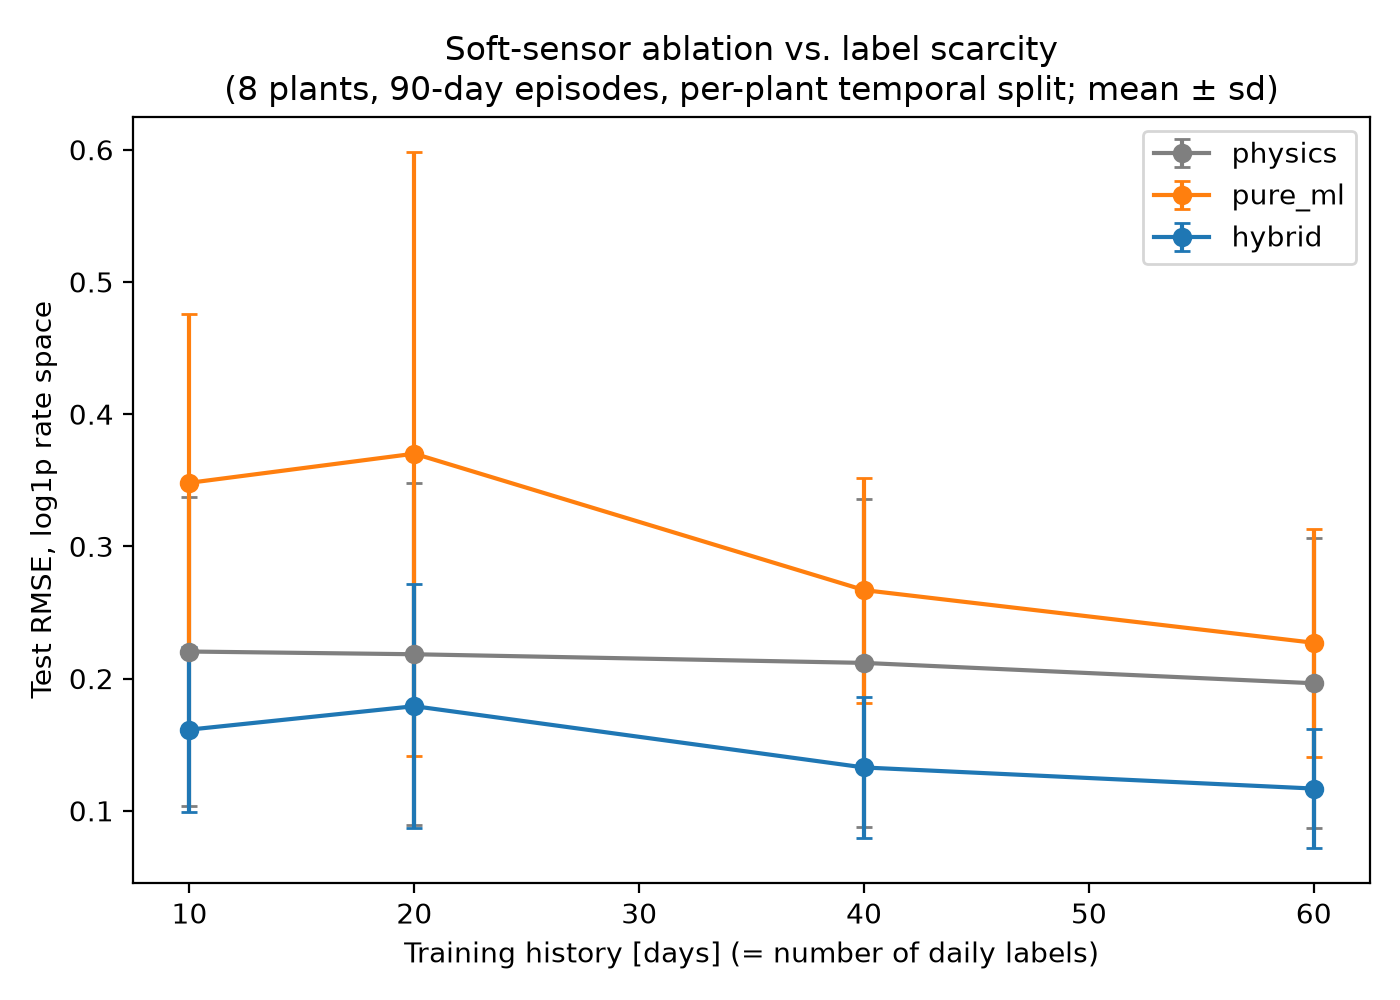
\includegraphics[width=.7\linewidth]{fig_scarcity_sweep.png}
\caption{Test RMSE versus training-history length, equal to the number
of daily labels; mean $\pm$ sd over 8 plants. Source:
\texttt{results/scarcity\_sweep.csv}.}\label{fig:scarcity}
\end{figure}

\subsection{Closed loop under benign mismatch}\label{sec:table2}

Table~\ref{tab:control} reports the four-arm closed-loop benchmark on
six plants over 45 days each: a fixed empirical-practice baseline at
150~$^{\circ}$C and 1~ppm continuous dosing, the pattern of documented
field programs~\citep{baltazar2014grc}; the vertex-robust RTO without
feedback; the scalar-MA loop; and the proposed hybrid-in-the-loop
controller.
% SOURCE: results/table2_summary.csv
\begin{table}[t]\centering
\caption{Closed-loop benchmark in the benign regime (random per-plant
mismatch; 6 plants $\times$ 45 d). Violation days count days whose
realized trailing-24-h mean rate exceeded $r_{\max}$.
Source: \texttt{results/table2\_summary.csv}.}
\label{tab:control}
\begin{tabular}{lcccc}
\toprule
Arm & Gross MW & Uplift & Viol.\ days (max) & Inhib.\ PHP/MWh \\
\midrule
Baseline (fixed) & 5.03 & --- & 0.00 (0) & 85.9 \\
RTO, no feedback & 7.12 & $+41.7\%$ & 0.17 (1) & 51.6 \\
RTO + scalar MA & 9.26 & $+84.1\%$ & 5.33 (12) & 41.2 \\
RTO + hybrid, $\kappa{=}1$ & 6.71 & $+33.4\%$ & \textbf{0.00 (0)} & 53.5 \\
\bottomrule
\end{tabular}
\end{table}
Three observations follow. Even the robust open-loop RTO leaks: one
plant, one violation day, because an envelope over brine chemistry does
not certify against kinetic draws. The scalar-MA loop harvests
spectacularly and unsafely, posting $+84\%$ uplift at an average of
5.33 violation days per plant and twelve on the worst plant, in the
benign regime. The hybrid controller is violation-free on all six
plants; its $+33\%$ uplift sits 8 percentage points below the
no-feedback RTO, and that gap is the premium of the $\kappa\sigma$
back-off. It is the price of insurance, quantified.

\subsection{Adverse-kinetics stress}\label{sec:stress}

The stress magnitude is a measurement, not a choice. The out-of-sample
validation of Section~\ref{sec:validation} finds a sixfold median gap
between the fitted core and independent modern kinetics, so the stress
sets the plant's true rate six times above the model as a deterministic
single-factor perturbation with all random draws zeroed.
Table~\ref{tab:stress} reports the pre-registered outcome.
% SOURCE: results/table2b_summary.csv
\begin{table}[t]\centering
\caption{Adverse stress at the measured sixfold kinetic gap
(single-factor; 6 plants $\times$ 45 d). ``Post-w.'' counts violation
days after the 8-day warm-up. Source:
\texttt{results/table2b\_summary.csv}.}
\label{tab:stress}
\begin{tabular}{lcccc}
\toprule
Arm & Uplift & Viol.\ days & Post-w. & Net kPHP/h \\
\midrule
Baseline (fixed) & --- & 0.00 & 0.00 & 27.2 \\
RTO, no feedback & $+41.7\%$ & 20.67 & 17.17 & 38.8 \\
RTO + scalar MA & $+37.0\%$ & 16.50 & 14.17 & 37.5 \\
RTO + hybrid, $\kappa{=}0$ & $+21.0\%$ & 4.33 & 2.17 & 33.1 \\
RTO + hybrid, $\kappa{=}1$ & $+6.2\%$ & \textbf{2.67} & \textbf{0.50} & 29.1 \\
\bottomrule
\end{tabular}
\end{table}
The no-feedback RTO violates chronically, on 17.2 of 37 post-warm-up
days: its vertex envelope covers brine uncertainty, not kinetic
mismatch. The scalar-MA loop barely improves on open loop (14.2), and
the mechanism is now precise. An additive bias correction learned at
one operating point cannot stabilize a multiplicative error on a
quartic constraint; the absolute error it measures is small when the
plant runs hot and explodes when the optimizer moves cold, so the loop
hunts and violates in a limit cycle. The hybrid constraint, being
state-dependent, extrapolates structurally. Even without margin
($\kappa{=}0$) it cuts post-warm-up violations eightfold, to 2.17 days.
Our pre-registered target for that arm was zero, and it was not met; we
report the miss. The uncertainty back-off ($\kappa{=}1$) closes the
remainder to 0.50 days at a further harvest cost, which we read as an
honest frontier point: under a sixfold kinetic error there is little
harvest that is safe to take. We also observe the optimizer
substituting the dose lever for the temperature lever once the latter
becomes risk-expensive, with inhibitor intensity falling to
38--45~PHP/MWh on several stressed plants. Across both regimes the
conclusion is a two-by-two. Open-loop robustness is safe but blind,
scalar adaptation is reactive but unsafe, and only the
credibility-weighted hybrid with back-off remains essentially
violation-free in both.

\subsection{Global sensitivity and economic ranges}\label{sec:sobol}

A Sobol study ($N = 512$, seeded, 9{,}216 evaluations) spans the
declared uncertainty set: a kinetic band equal to the measured sixfold
gap, a solubility band equal to the measured endpoint spread
$[0.90, 1.37]$, and declared scenario bands for flash, dose--response,
$r_{\max}$ and economics (Fig.~\ref{fig:sobol}). Kinetic model-family
uncertainty dominates the economics, with total-order indices of 0.41,
0.57 and 0.33 on gross power, optimal temperature and net objective.
The quantity the sensing layer reduces is the quantity that moves the
money. The optimal dose is governed instead by dose--response knowledge
($S_T = 0.67$), which identifies inhibitor characterization as the
second identification target. Feasibility holds at 100\% across the
set, so the declared uncertainty never strands the optimizer, and the
gross-power optimum spans 6.0/11.7/17.6~MW
($q_{05}/q_{50}/q_{95}$). Finally, re-valuing the committed closed-loop
trajectories over the economics envelope attaches ranges to every peso
figure. The enabling assumption is verified rather than assumed: the
optimum moves zero grid steps across all eight envelope corners, with
inhibitor cost below 15\% of revenue everywhere, so uplift percentages
and violation counts are untouched. The safety conclusions of
Tables~\ref{tab:control} and~\ref{tab:stress} do not depend on economic
assumptions.

\begin{figure}[t]\centering
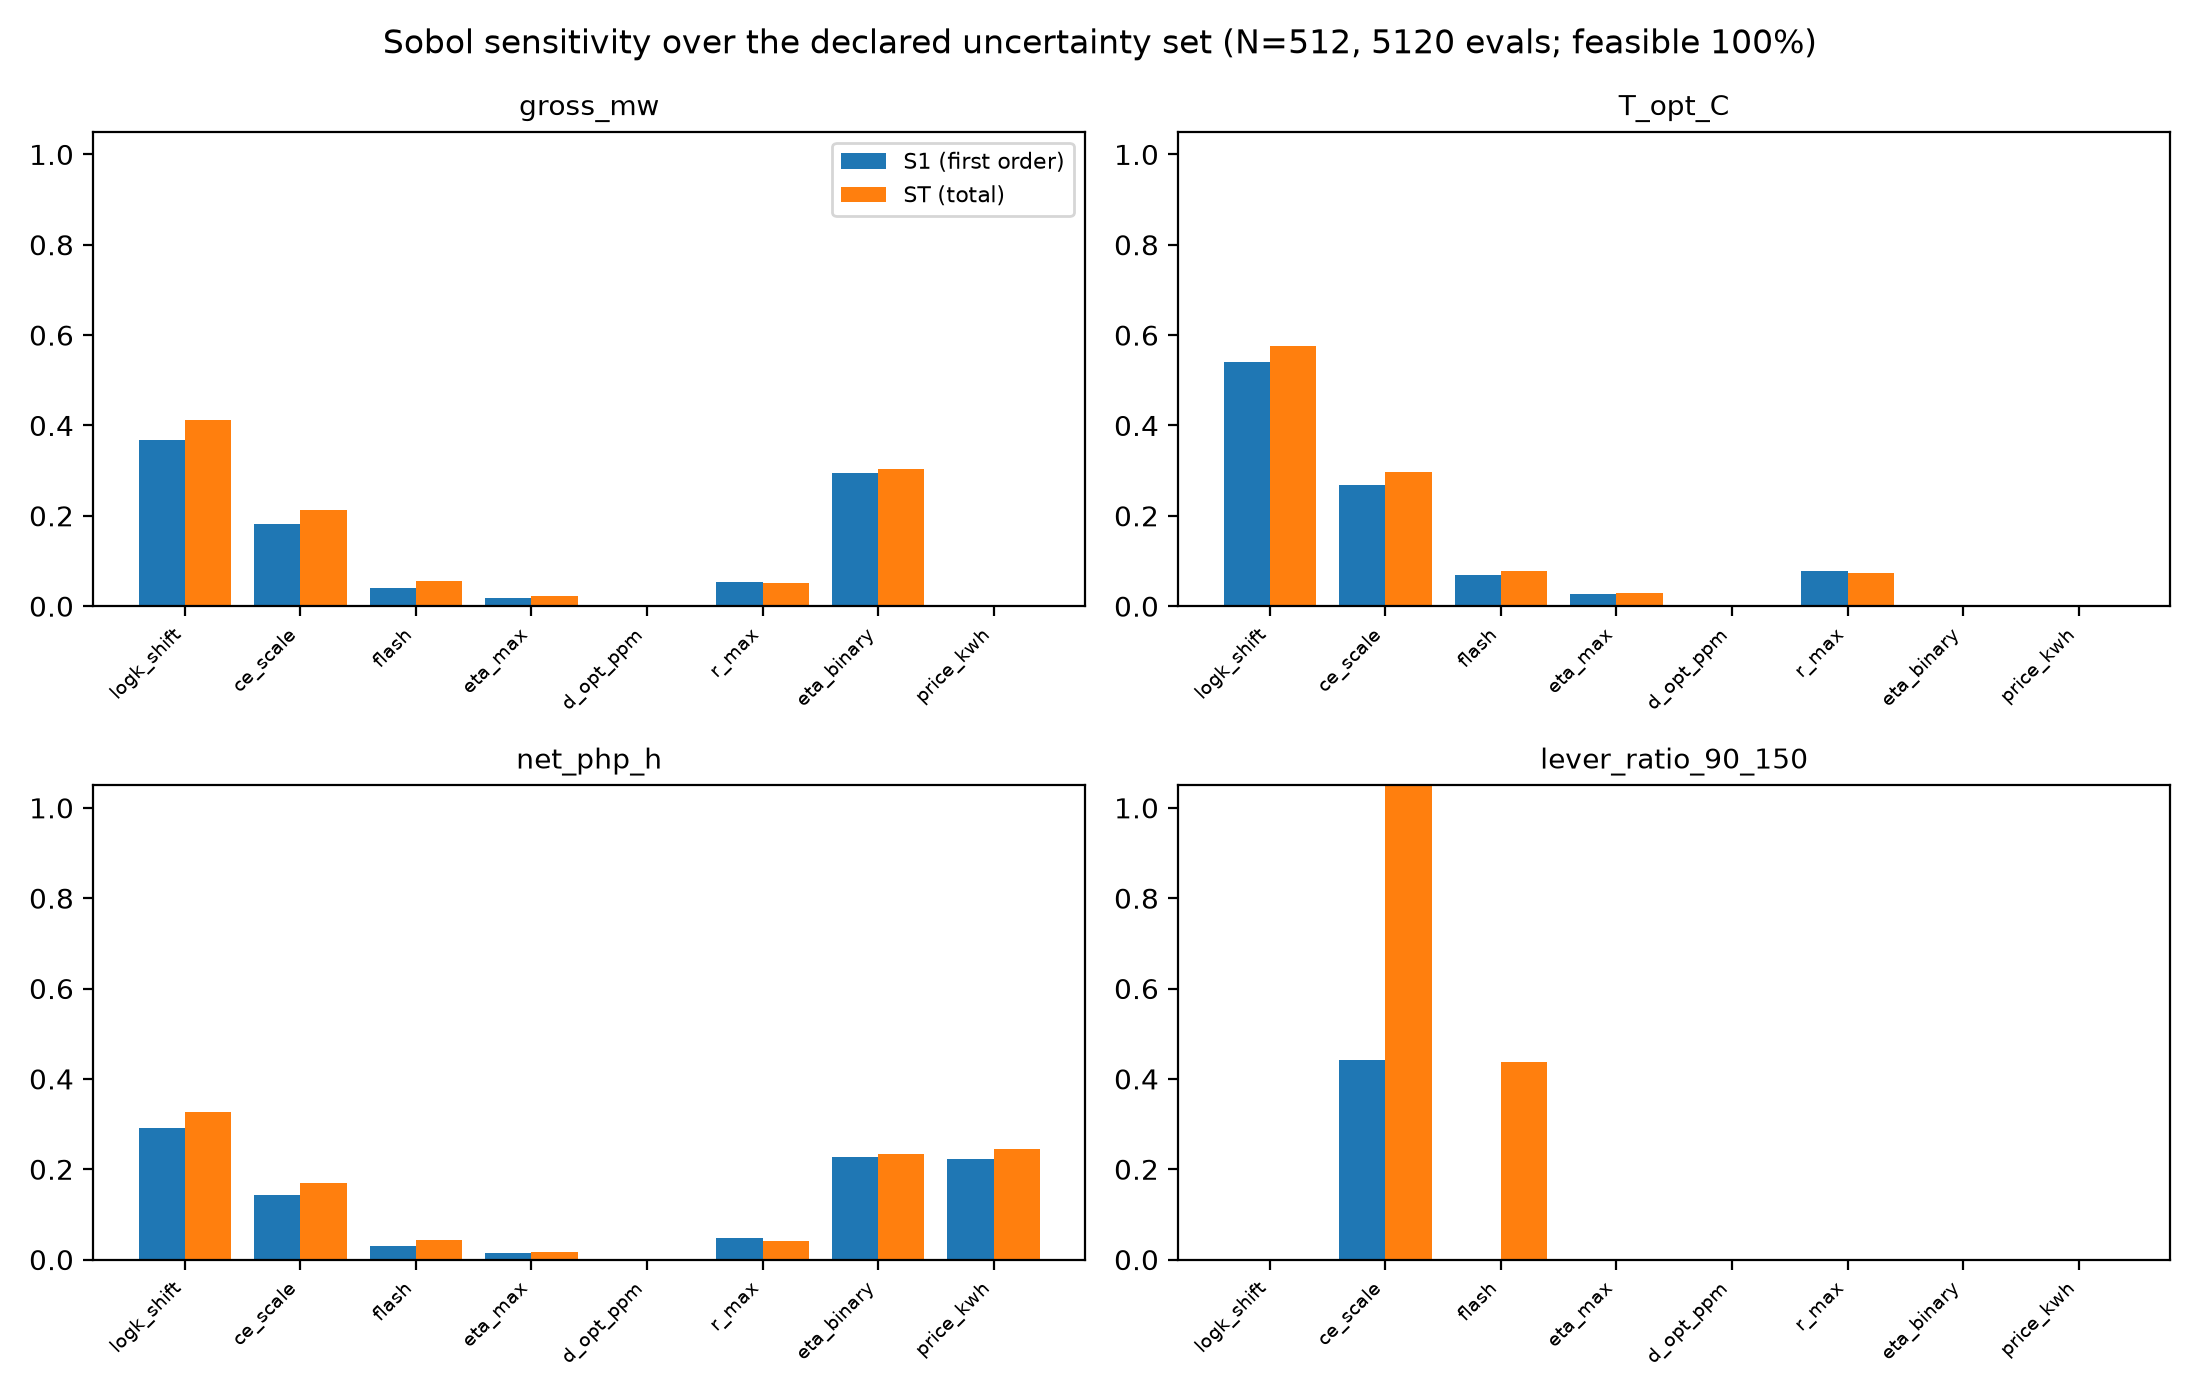
\includegraphics[width=.95\linewidth]{fig_sensitivity_sobol.png}
\caption{First- and total-order Sobol indices over the declared
uncertainty set. Source: \texttt{results/sensitivity\_sobol.csv}.}
\label{fig:sobol}
\end{figure}

\section{Out-of-sample validation on independent data}\label{sec:validation}

Every physics component of the architecture, and the sensing pattern
itself, is confronted with an experimental dataset it was never fitted
to: the supplementary data of \citet{scott2024silica}, read with the
parameterization corrections of \citet{scott2024corrigendum}. The
corpus comprises 61 monomeric-silica decay experiments and 1{,}275
points spanning 23--80~$^{\circ}$C, pH 2.1--10.0 and ionic strength
0.01--0.53~mol/kg. Because the source is machine-readable, manual
transcription protocols give way to automated parser integrity checks:
unit-header pinning, monotonicity, separation of replicate runs listed
under duplicated identifiers, and flagging of one colloid-regime
outlier that falls outside the dissolved-monomer scope.

\subsection{Kinetics: what a 1979 law does and does not predict}

Two properties of the fitted core are tested separately, because they
fail differently. Consider first the functional form. Linearizing the
integrated $n$-th-order decay law and sweeping $n \in \{2,\dots,6\}$
per experiment shows that single-curve monomer decay in the modern data
is cleanly second order in supersaturation: median $R^2 = 0.992$ at
$n = 2$, degrading monotonically as the assumed order rises, with
best-fit order 2 in all eleven qualifying near-neutral experiments
(Fig.~\ref{fig:kinval}). This does not contradict the source of the
core. The classical ``fourth order'' is a correlation of maximum rate
against initial supersaturation across separate batches, a peak-rate
law, whereas the integrated decay of a single curve follows
Rimstidt--Barnes-type second-order
kinetics~\citep{rimstidt1980kinetics}. The two describe different
observables, and we report both rather than forcing either onto data
that says otherwise. Now the rate level. The observed second-order
constants follow an Arrhenius trend with $E_a \approx 22$~kJ/mol, and
the effective decay constant implied by the fitted core differs from
observation by a factor of about six at the median. That number does
double duty in this paper. It calibrates the adverse stress of
Section~\ref{sec:stress}, and it is the measured size of the gap the
learned residual exists to absorb: no single transcribed rate law
reproduces independent modern data.

\begin{figure}[t]\centering
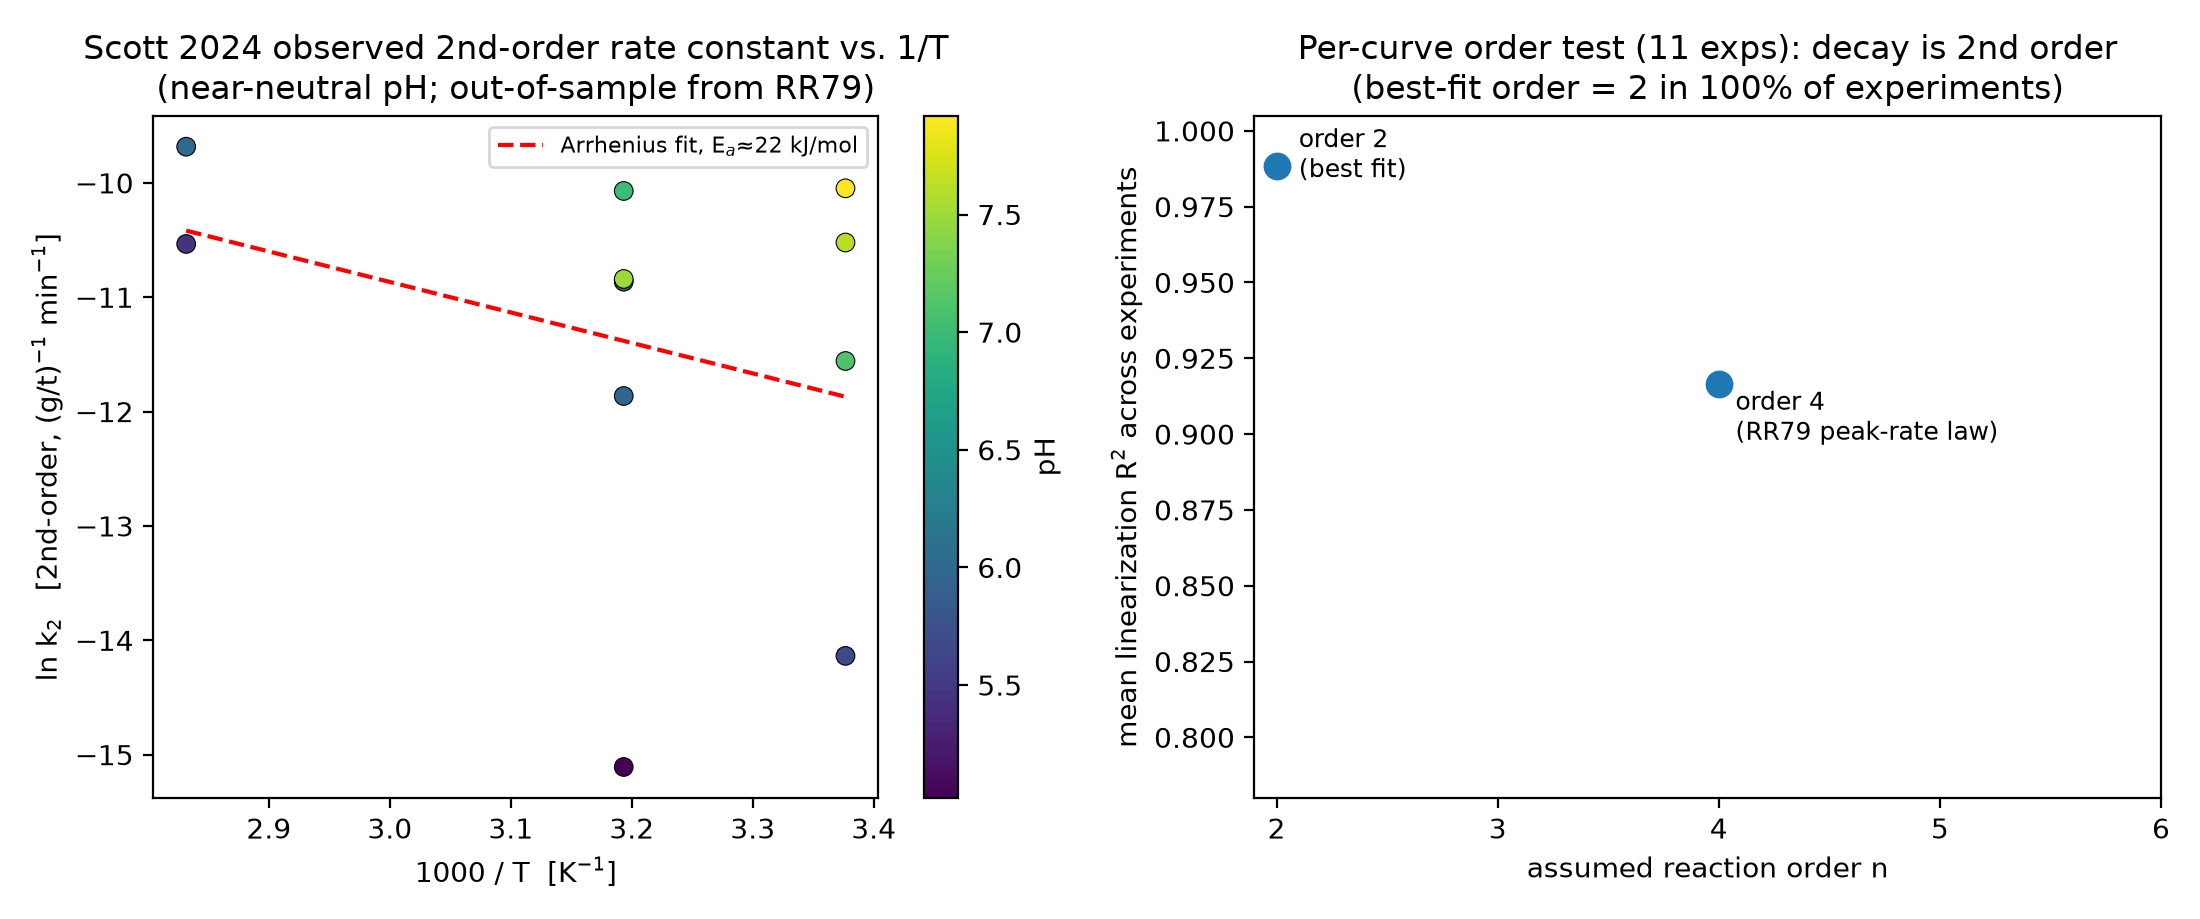
\includegraphics[width=.95\linewidth]{fig_kinetics_validation.png}
\caption{Out-of-sample kinetic validation against
\citet{scott2024silica}. Left: observed second-order rate constants
versus inverse temperature for the near-neutral experiments, with the
Arrhenius trend. Right: mean linearization $R^2$ versus assumed
reaction order; single-curve decay is second order, while the
fourth-order form is a peak-rate law. Source:
\texttt{results/kinetics\_validation.csv}.}
\label{fig:kinval}
\end{figure}

\subsection{Solubility: mutual validation across 24 years}

The plateau of a near-complete decay experiment is an independent
measurement of amorphous-silica solubility. Sixteen near-neutral
experiments that consumed at least 70\% of their initial
supersaturation plateau at 0.90--1.37 times the
\citet{gunnarsson2000amorphous} correlation, with a median of 1.05. The
2000 correlation and the 2024 endpoints therefore validate each other
in both directions, and the measured band $[0.90, 1.37]$ becomes the
solubility axis of the sensitivity study in Section~\ref{sec:sobol}.

\subsection{The sensing pattern on real curves: identifiability
precedes correction}\label{sec:sensorval}

Finally, the field sensing pattern is replayed on laboratory truth.
Each qualifying experiment is treated as a plant, interval-average
observed rates as the hidden truth, the fitted core as the prior, and
only the first $K$ intervals as labels. Three arms with honestly
counted parameters are compared: the core alone; a one-parameter scalar
hybrid, a fitted log-level offset that is deployable from a single
label, where a data-only fit cannot operate at all; and a two-parameter
affine hybrid whose slope in $\ln s$ is, by construction, an order
correction. Second-order truth against a fourth-order core predicts
$b \approx -2$.

The raw affine arm is retained as a cautionary ablation. Early labels
span almost no state (a label $\ln s$ spread of 0.047 against a test
span of 2.61), so unregularized slopes explode, with $b$ ranging from
$-230$ to $+769$, and the arm performs far worse than no correction at
all. Applying the same credibility mechanism as the field sensor, a
leave-one-out selection between the scalar and a clipped affine, the
correction collapses to the safe scalar whenever the labels have not
earned the slope ($K \le 3$). At $K = 5$ it engages in 9 of 21
experiments with median $b = -2.50$, independently re-measuring the
order-2 finding, and wins outright with a median RMSE of 2.59 against
3.04 for the core (Fig.~\ref{fig:sensorval}). The principle this
crystallizes, identifiability precedes correction, also explains the
field results. A plant regulated near an operating point presents a
level-dominated, label-covered correction problem, which is exactly
where hybrid residuals win; wide-range extrapolation demands
state-spanning labels, and a credible architecture must know which
regime it is in.

\begin{figure}[t]\centering
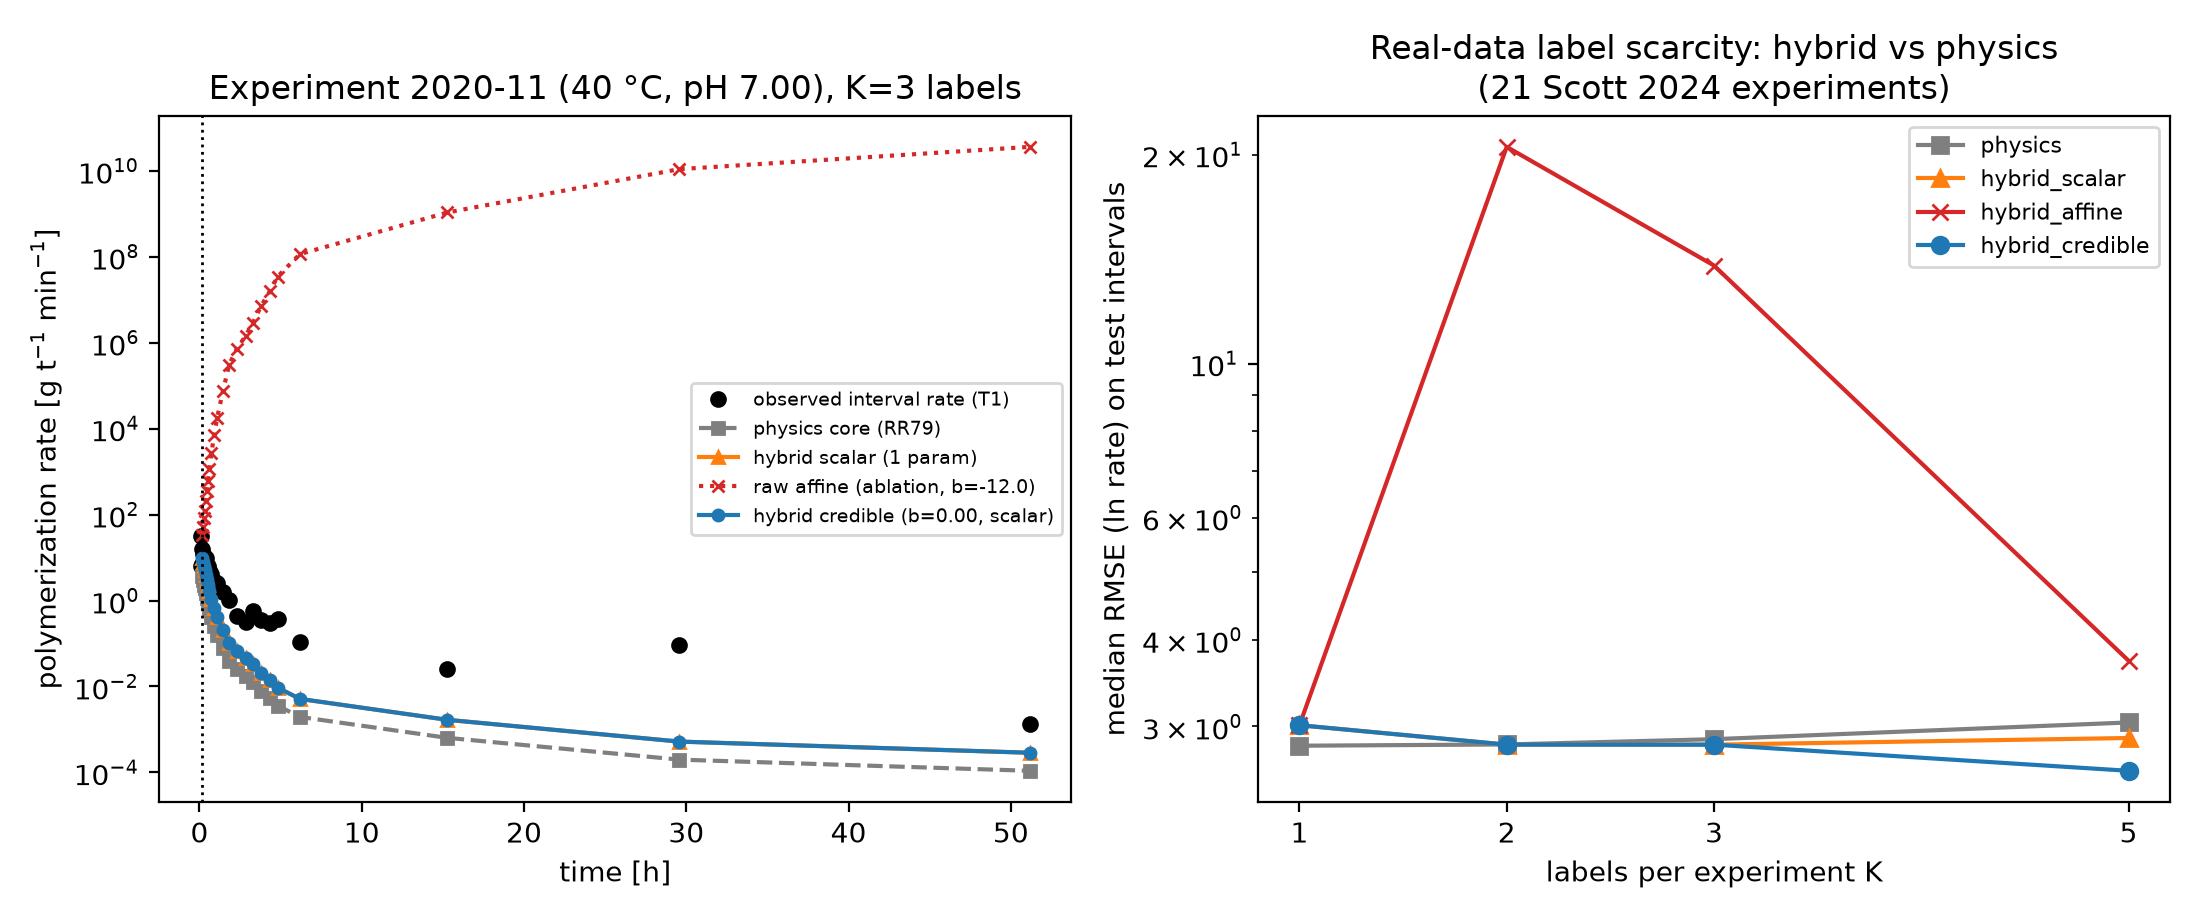
\includegraphics[width=.95\linewidth]{fig_sensor_validation_scott.png}
\caption{The sensing pattern on real decay curves. Left: a
representative experiment, showing the observed interval rates, the
diverging physics core, the raw-affine explosion, and the credible
hybrid. Right: median test RMSE versus labels per experiment $K$ for
all arms, on a log scale. Source:
\texttt{results/sensor\_validation\_scott.csv}.}
\label{fig:sensorval}
\end{figure}

\section{Discussion and limitations}\label{sec:discussion}

\paragraph{Evaluation posture.} The closed-loop results are in silico.
The plant is synthetic, though every physical ingredient, from
solubility and kinetics to the brine envelope and the actuator family,
is grounded in primary literature and, wherever independent data
exists, validated out-of-sample component by component
(Section~\ref{sec:validation}). We regard component-wise real-data
validation combined with a parameterized-mismatch closed loop as the
honest intermediate between simulation-only studies and a field trial.
A field pilot is the natural next step, and it would require exactly
the sparse instrumentation this architecture is designed around.

\paragraph{Constraint units.} The scaling constraint is expressed as a
polymerization (monomer-depletion) rate rather than a wall-deposition
thickness rate. The molecular-deposition treatment of
\citet{weres1981kinetics}, transcribed under the same integrity
protocol (its printed checkpoints reproduce, including the 3.0~kcal/mol
effective activation energy; one internal inconsistency in its
Eq.~[4c] is documented rather than silently repaired), closes the unit
gap. Along the envelope where the constraint is active,
$r_{\max} = 0.5$~g\,t$^{-1}$\,min$^{-1}$ corresponds to a Weres-implied
molecular-deposition wall growth, a lower bound on total scale growth,
of about 0.3~mm/yr at the optimized operating point and 0.04 to
1.6~mm/yr across 90--175~$^{\circ}$C; the four-fold $r_{\max}$ band of
the sensitivity study spans that calibration.

\paragraph{Scenario fencing.} Trade-press figures inform scenario scale
only. The rule is enforced mechanically in the repository, and every
peso and megawatt headline carries an envelope range with decision
invariance verified rather than assumed.

\paragraph{Design constants.} The back-off gain is fixed at
$\kappa = 1$. Its ablation over $\kappa \in \{0,1\}$ brackets the
safety--harvest trade under stress, and $\sigma_{\mathrm{LOO}}$ is
already data-adaptive. A continuous $\kappa$ sweep is the tuning study we
would prioritize next.

\paragraph{Scope boundaries.} High-pH brines require silica ionization
corrections that are deferred here; the speciation layer exists in the
repository but is not exercised in the loop. The identifiability
principle of Section~\ref{sec:sensorval} is likewise a scope statement
rather than a weakness: corrections are used only where labels can
support them, and the architecture knows which regime it is in.

\paragraph{What generalizes.} Nothing in
Eqs.~\eqref{eq:sensor}--\eqref{eq:rto} is specific to silica. The
pattern, a physics prior corrected only to its earned credibility and
feeding a constraint backed off by the correction's own cross-validated
uncertainty, applies to any hard-constrained process operated against a
structurally wrong model: fouling, crystallization, corrosion, membrane
scaling. Geothermal silica supplies an unusually clean and unusually
demanding instance, with quartic constraint sensitivity, an induction
delay, non-monotonic actuation, and a measured sixfold model-family
gap, and that is why we offer it as a benchmark.

\section{Conclusions}\label{sec:conclusions}

We posed geothermal silica scaling as what it is for a control
engineer: a hard-constrained economic optimization run against a model
known to be structurally wrong, with the size of the wrongness measured
at a sixfold median gap against independent modern kinetics rather than
assumed. The architecture answers mismatch with two coupled mechanisms,
a hybrid soft sensor whose learned correction is weighted by its own
leave-one-out credibility, and a vertex-robust economic real-time
optimizer that consumes both the correction and its uncertainty as a
constraint back-off. Under sparse daily labels the sensor cuts
estimation error by 40\% against its physics prior and by 48\% against
a pure-data baseline. In closed loop it is the only tested policy that
remains essentially free of constraint violations in both regimes:
benign mismatch, at $+33\%$ power uplift with zero violation days on
six of six plants, and a stress set at the measured sixfold gap, at
0.50 post-warm-up violation days against 17.2 for the robust open
loop. Two pre-registered failures shaped the design and are reported
as results. Zero-shot residual transfer harms, which makes earned
credibility the deployment interlock; and scalar modifier adaptation
cannot stabilize a multiplicative error on a quartic constraint, which
makes state-dependent correction necessary rather than merely
preferable. Every physics component, and the sensing pattern itself,
was validated out-of-sample. That exercise returned two findings of
independent geochemical interest, that single-curve decay is second
order against the classical fourth-order peak-rate law and that the
2000 solubility correlation and the 2024 endpoints mutually validate
at a median of $1.05\times$, together with one transferable design
principle: identifiability precedes correction.

\section*{Data and code availability}
The complete repository, comprising the primary-data transcriptions
with integrity checks, all models, experiments and figures, regenerates
every result through a single gate script (94 automated checks across
13 modules, deterministic seeds throughout). An archival release is
planned upon acceptance. A third-party author-provided reference script
is excluded pending its author's permission.


\section*{Acknowledgments}
The author thanks Dr.~Samuel Scott for directing him to the study's
supplementary dataset, for clarifying the published parameterization
and its corrigendum, and for providing a reference implementation
script used for cross-checking, which is not redistributed with this
work. This work received no external funding.

\appendix
\section{Data transcription and integrity protocol}\label{app:protocol}
Primary numerical sources enter the repository only through a
transcription protocol: tables are transcribed to CSV against the
publisher's text layer, validated against printed derived quantities
where the source provides them (for the kinetic dataset of
\citet{rothbaum1979rohde}, the printed $R \cdot P^{1.5}$ checksum column
validates 33 of 33 retained rows; one flagged row is excluded), and
tagged with an evidence tier: T1 for peer-reviewed primary sources, T2
for conference or institutional material, and T3 for trade press, which
may motivate scenario scale only and is never fitted, a rule enforced
in code. Machine-readable sources
replace manual transcription with automated parser integrity checks
(Section~\ref{sec:validation}).

\section{Reproducibility}\label{app:repro}
A single gate script executes the self-checks of all twelve modules
(94 checks at the time of writing) and refuses a green status unless
every check passes; the repository convention is that no commit is made
against a red gate, and all figures and result tables regenerate from
source and raw transcriptions. All stochastic components are seeded,
including the Sobol sampler, whose default scrambled quasi-random
sequence is pinned for run-to-run reproducibility. The Python
environment is pinned in \texttt{requirements.txt}; principal
dependencies are NumPy/SciPy/pandas, LightGBM~\citep{ke2017lightgbm},
SALib~\citep{herman2017salib}, and PHREEQC via
phreeqpython~\citep{parkhurst2013phreeqc} for the (deferred) speciation
layer.


\bibliographystyle{elsarticle-num}
\bibliography{references}   % copied in by compile.bat from /literature

\end{document}
